% ExVA/Lego/256:     u4108 -> lego_random_exr
%       150k:   24.00 & 0.88 & 0.101 & 0.207 & 150k & 256px & 11h30m
%       80k:    23.76 & 0.87 & 0.117 & 0.215 & 80k & 256px & 5h
% ImNRF/Lego/256:     u4107 -> lego_random_exr

\begingroup
\begin{figure}[!htb]
    % \setArraystrech{1.5}
    \centering
    \setlength\tabcolsep{0pt}
    \begin{tabular*}{\textwidth}{ c c c c c }
        Target & ImNRF & ExVA & ImNRF\textsubscript{HDRFlip} & ExVA\textsubscript{HDRFlip} \\
        % \multicolumn{2}{c}{256px} & 256px & \multicolumn{2}{c}{64px} \\
        % 256px & 256px & 256px & 64px & 64px \\
        
          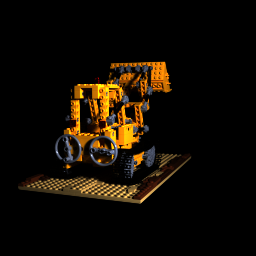
\includegraphics[width=0.2\textwidth]{figures/results/arb_set/validation/lego6_targ_256px.png}
        & 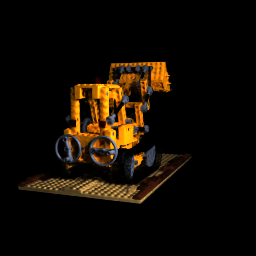
\includegraphics[width=0.2\textwidth]{figures/results/arb_set/validation/lego6_imnrf_150k.png}
        & 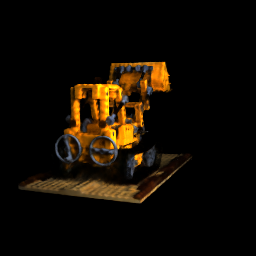
\includegraphics[width=0.2\textwidth]{figures/results/arb_set/validation/lego6_exva_150k.png}
        & 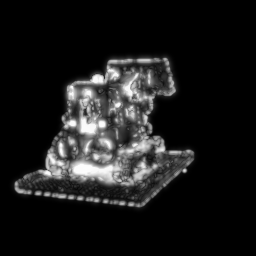
\includegraphics[width=0.2\textwidth]{figures/results/arb_set/validation/lego6_imnrf_hdrflip_150k.png}
        & 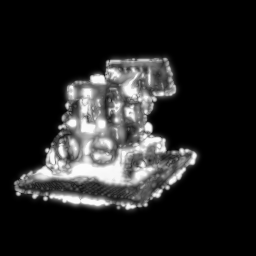
\includegraphics[width=0.2\textwidth]{figures/results/arb_set/validation/lego6_exva_hdrflip_150k.png} \\[-6pt]
        
          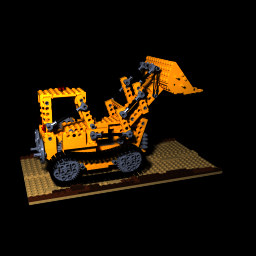
\includegraphics[width=0.2\textwidth]{figures/results/arb_set/validation/lego7_targ_256px.png}
        & 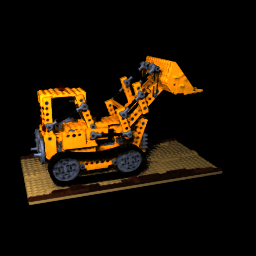
\includegraphics[width=0.2\textwidth]{figures/results/arb_set/validation/lego7_imnrf_150k.png}
        & 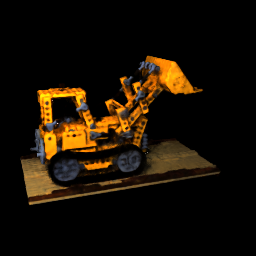
\includegraphics[width=0.2\textwidth]{figures/results/arb_set/validation/lego7_exva_150k.png}
        & 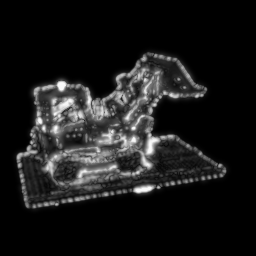
\includegraphics[width=0.2\textwidth]{figures/results/arb_set/validation/lego7_imnrf_hdrflip_150k.png}
        & 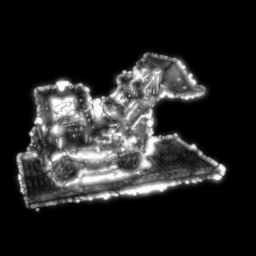
\includegraphics[width=0.2\textwidth]{figures/results/arb_set/validation/lego7_exva_hdrflip_150k.png} \\[-6pt]
        
          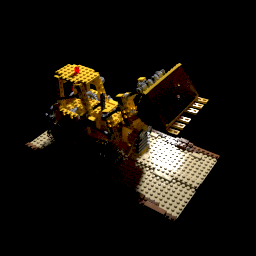
\includegraphics[width=0.2\textwidth]{figures/results/arb_set/validation/lego10_targ_256px.png}
        & 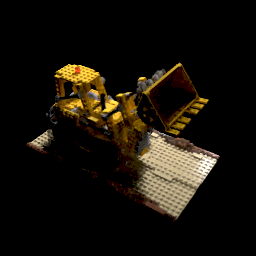
\includegraphics[width=0.2\textwidth]{figures/results/arb_set/validation/lego10_imnrf_150k.png}
        & 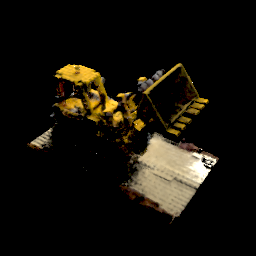
\includegraphics[width=0.2\textwidth]{figures/results/arb_set/validation/lego10_exva_150k.png}
        & 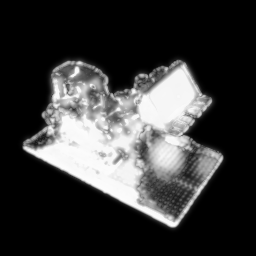
\includegraphics[width=0.2\textwidth]{figures/results/arb_set/validation/lego10_imnrf_hdrflip_150k.png}
        & 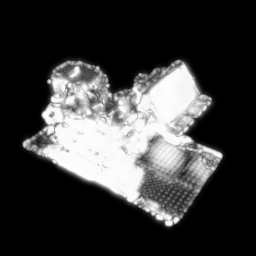
\includegraphics[width=0.2\textwidth]{figures/results/arb_set/validation/lego10_exva_hdrflip_150k.png} \\[-6pt]
        
          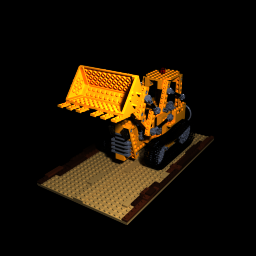
\includegraphics[width=0.2\textwidth]{figures/results/arb_set/validation/lego14_targ_256px.png}
        & 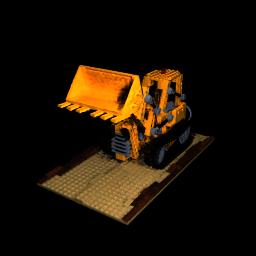
\includegraphics[width=0.2\textwidth]{figures/results/arb_set/validation/lego14_imnrf_150k.png}
        & 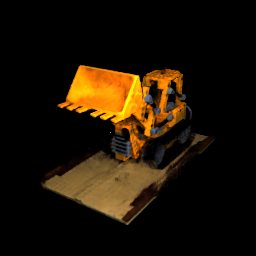
\includegraphics[width=0.2\textwidth]{figures/results/arb_set/validation/lego14_exva_150k.png}
        & 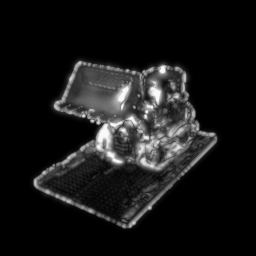
\includegraphics[width=0.2\textwidth]{figures/results/arb_set/validation/lego14_imnrf_hdrflip_150k.png}
        & 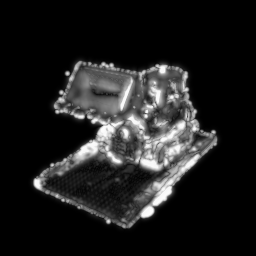
\includegraphics[width=0.2\textwidth]{figures/results/arb_set/validation/lego14_exva_hdrflip_150k.png}
        

    \end{tabular*}
    \caption{The overview of some novel light-view synthesis results
    achieved with our methods trained on arbitrary light setting Lego dataset
    for 150k iterations using 256px images.
    Each row correspond to one specific novel light-view location,
    second and third columns show synthesized images,
    last two columns contain difference images
    calculated between corresponding predictions and target images using HDRFlipLoss (\Cref{sec:metrics}).
    Renders from the third row have been post-processed (gamma-correction with $\gamma = 2.5$ and scaling)
    since the original view is very dark with very bright spot from the reflection of the light source.
    Note that \textit{ImNRF} was able to better reproduce fine details.
    Both methods fail to predict highly specular spot on the third row.
    }
    \label{tab:arb_selective_results}
\end{figure}
\endgroup